\documentclass{standalone}
\usepackage{tikz}
\usetikzlibrary{patterns, positioning}

\begin{document}
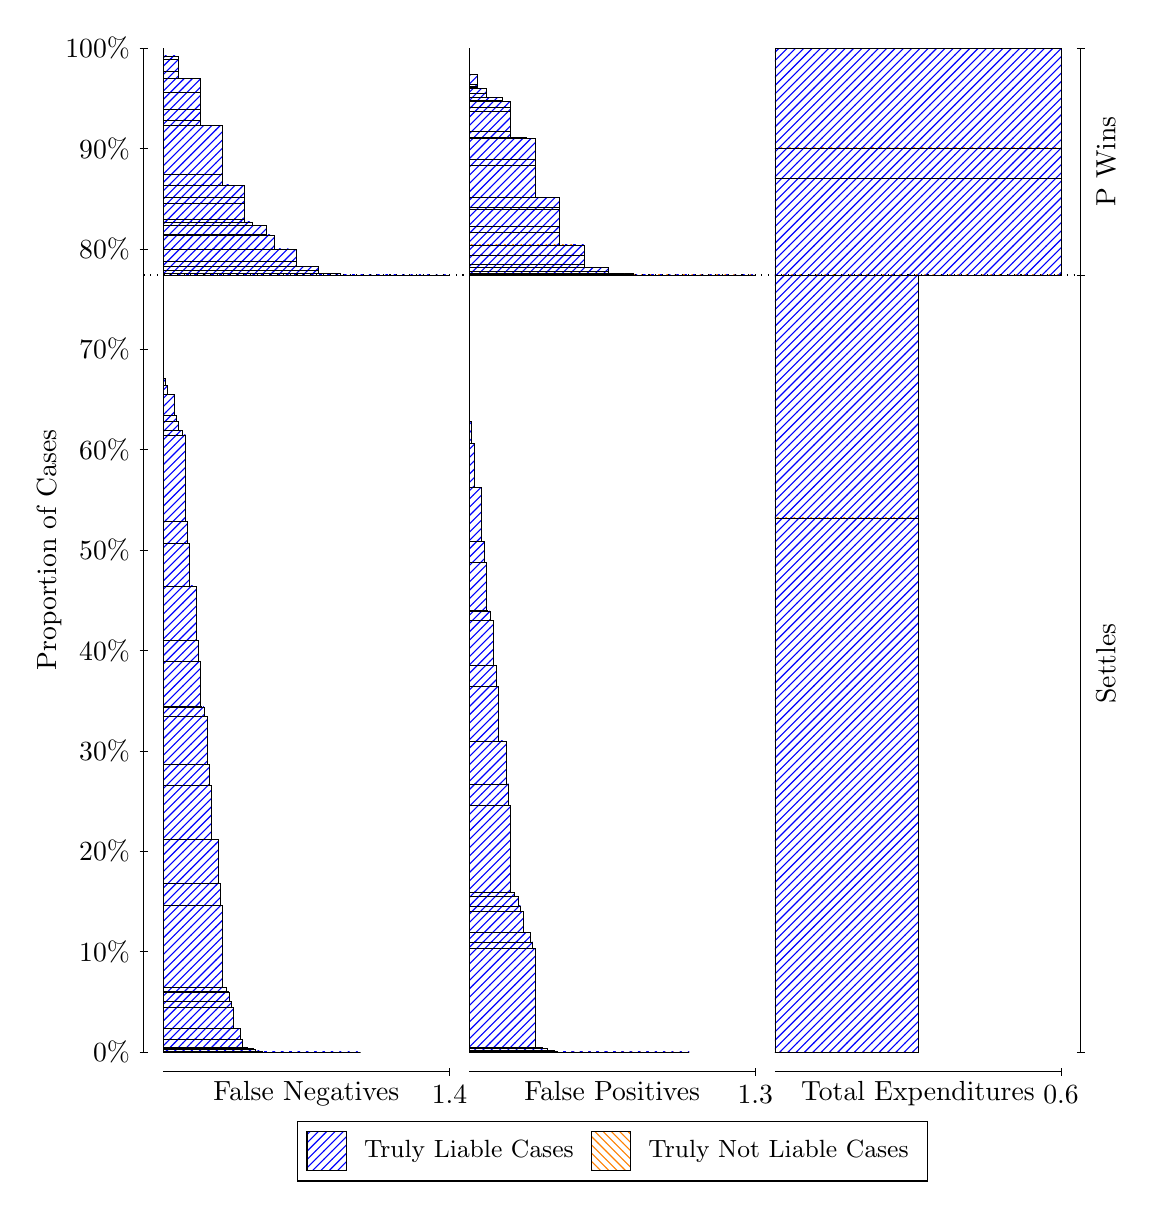
\begin{tikzpicture}
\draw[black, very thin] (1.5,1.75) -- (1.5,14.5);
\node[rotate=90, anchor=center] at (0.3, 8.125) {Proportion of Cases};
\draw[black, very thin] (1.45,1.75) -- (1.55,1.75);
\node[anchor=east] at (1.45, 1.75) {0\%};
\draw[black, very thin] (1.45,3.025) -- (1.55,3.025);
\node[anchor=east] at (1.45, 3.025) {10\%};
\draw[black, very thin] (1.45,4.3) -- (1.55,4.3);
\node[anchor=east] at (1.45, 4.3) {20\%};
\draw[black, very thin] (1.45,5.575) -- (1.55,5.575);
\node[anchor=east] at (1.45, 5.575) {30\%};
\draw[black, very thin] (1.45,6.85) -- (1.55,6.85);
\node[anchor=east] at (1.45, 6.85) {40\%};
\draw[black, very thin] (1.45,8.125) -- (1.55,8.125);
\node[anchor=east] at (1.45, 8.125) {50\%};
\draw[black, very thin] (1.45,9.4) -- (1.55,9.4);
\node[anchor=east] at (1.45, 9.4) {60\%};
\draw[black, very thin] (1.45,10.675) -- (1.55,10.675);
\node[anchor=east] at (1.45, 10.675) {70\%};
\draw[black, very thin] (1.45,11.95) -- (1.55,11.95);
\node[anchor=east] at (1.45, 11.95) {80\%};
\draw[black, very thin] (1.45,13.225) -- (1.55,13.225);
\node[anchor=east] at (1.45, 13.225) {90\%};
\draw[black, very thin] (1.45,14.5) -- (1.55,14.5);
\node[anchor=east] at (1.45, 14.5) {100\%};

\draw[black, very thin] (13.4,1.75) -- (13.4,14.5);
\draw[black, very thin] (13.35,1.75) -- (13.45,1.75);
\node[anchor=west] at (13.35, 1.75) {};
\draw[black, very thin] (13.35,11.618) -- (13.45,11.618);
\node[anchor=west] at (13.35, 11.618) {};
\draw[black, very thin] (13.35,14.5) -- (13.45,14.5);
\node[anchor=west] at (13.35, 14.5) {};

\draw[black, very thin, pattern color=blue, pattern=north east lines] (1.75,1.75) rectangle (4.2557,1.75);
\draw[black, very thin, pattern color=blue, pattern=north east lines] (1.75,1.75) rectangle (4.0052,1.75);
\draw[black, very thin, pattern color=blue, pattern=north east lines] (1.75,1.75) rectangle (3.9773,1.75);
\draw[black, very thin, pattern color=blue, pattern=north east lines] (1.75,1.75) rectangle (3.7546,1.75);
\draw[black, very thin, pattern color=blue, pattern=north east lines] (1.75,1.75) rectangle (3.7268,1.75);
\draw[black, very thin, pattern color=blue, pattern=north east lines] (1.75,1.75) rectangle (3.6989,1.75);
\draw[black, very thin, pattern color=blue, pattern=north east lines] (1.75,1.75) rectangle (3.6293,1.75);
\draw[black, very thin, pattern color=blue, pattern=north east lines] (1.75,1.75) rectangle (3.4762,1.75);
\draw[black, very thin, pattern color=blue, pattern=north east lines] (1.75,1.75) rectangle (3.4483,1.75);
\draw[black, very thin, pattern color=blue, pattern=north east lines] (1.75,1.75) rectangle (3.4205,1.75);
\draw[black, very thin, pattern color=blue, pattern=north east lines] (1.75,1.75) rectangle (3.3787,1.75);
\draw[black, very thin, pattern color=blue, pattern=north east lines] (1.75,1.75) rectangle (3.3509,1.75);
\draw[black, very thin, pattern color=blue, pattern=north east lines] (1.75,1.75) rectangle (3.1978,1.7505);
\draw[black, very thin, pattern color=blue, pattern=north east lines] (1.75,1.7505) rectangle (3.1699,1.7506);
\draw[black, very thin, pattern color=blue, pattern=north east lines] (1.75,1.7506) rectangle (3.1421,1.7507);
\draw[black, very thin, pattern color=blue, pattern=north east lines] (1.75,1.7507) rectangle (3.1282,1.7507);
\draw[black, very thin, pattern color=blue, pattern=north east lines] (1.75,1.7507) rectangle (3.1003,1.7508);
\draw[black, very thin, pattern color=blue, pattern=north east lines] (1.75,1.7508) rectangle (3.0725,1.7508);
\draw[black, very thin, pattern color=blue, pattern=north east lines] (1.75,1.7508) rectangle (3.0029,1.7627);
\draw[black, very thin, pattern color=blue, pattern=north east lines] (1.75,1.7627) rectangle (2.9193,1.7888);
\draw[black, very thin, pattern color=blue, pattern=north east lines] (1.75,1.7888) rectangle (2.8915,1.7943);
\draw[black, very thin, pattern color=blue, pattern=north east lines] (1.75,1.7943) rectangle (2.8637,1.7999);
\draw[black, very thin, pattern color=blue, pattern=north east lines] (1.75,1.7999) rectangle (2.8497,1.8002);
\draw[black, very thin, pattern color=blue, pattern=north east lines] (1.75,1.8002) rectangle (2.8219,1.8052);
\draw[black, very thin, pattern color=blue, pattern=north east lines] (1.75,1.8052) rectangle (2.7941,1.8054);
\draw[black, very thin, pattern color=blue, pattern=north east lines] (1.75,1.8054) rectangle (2.7523,1.9166);
\draw[black, very thin, pattern color=blue, pattern=north east lines] (1.75,1.9166) rectangle (2.7245,2.0531);
\draw[black, very thin, pattern color=blue, pattern=north east lines] (1.75,2.0531) rectangle (2.6409,2.3172);
\draw[black, very thin, pattern color=blue, pattern=north east lines] (1.75,2.3172) rectangle (2.6131,2.391);
\draw[black, very thin, pattern color=blue, pattern=north east lines] (1.75,2.391) rectangle (2.5852,2.5123);
\draw[black, very thin, pattern color=blue, pattern=north east lines] (1.75,2.5123) rectangle (2.5713,2.5147);
\draw[black, very thin, pattern color=blue, pattern=north east lines] (1.75,2.5147) rectangle (2.5435,2.5678);
\draw[black, very thin, pattern color=blue, pattern=north east lines] (1.75,2.5678) rectangle (2.5156,2.5702);
\draw[black, very thin, pattern color=blue, pattern=north east lines] (1.75,2.5702) rectangle (2.5017,3.6107);
\draw[black, very thin, pattern color=blue, pattern=north east lines] (1.75,3.6107) rectangle (2.4739,3.8927);
\draw[black, very thin, pattern color=blue, pattern=north east lines] (1.75,3.8927) rectangle (2.446,4.4453);
\draw[black, very thin, pattern color=blue, pattern=north east lines] (1.75,4.4453) rectangle (2.3625,5.1353);
\draw[black, very thin, pattern color=blue, pattern=north east lines] (1.75,5.1353) rectangle (2.3347,5.4048);
\draw[black, very thin, pattern color=blue, pattern=north east lines] (1.75,5.4048) rectangle (2.3068,6.011);
\draw[black, very thin, pattern color=blue, pattern=north east lines] (1.75,6.011) rectangle (2.2929,6.0167);
\draw[black, very thin, pattern color=blue, pattern=north east lines] (1.75,6.0167) rectangle (2.2651,6.1333);
\draw[black, very thin, pattern color=blue, pattern=north east lines] (1.75,6.1333) rectangle (2.2372,6.1389);
\draw[black, very thin, pattern color=blue, pattern=north east lines] (1.75,6.1389) rectangle (2.2233,6.7102);
\draw[black, very thin, pattern color=blue, pattern=north east lines] (1.75,6.7102) rectangle (2.1955,6.9777);
\draw[black, very thin, pattern color=blue, pattern=north east lines] (1.75,6.9777) rectangle (2.1676,7.668);
\draw[black, very thin, pattern color=blue, pattern=north east lines] (1.75,7.668) rectangle (2.0841,8.214);
\draw[black, very thin, pattern color=blue, pattern=north east lines] (1.75,8.214) rectangle (2.0563,8.4868);
\draw[black, very thin, pattern color=blue, pattern=north east lines] (1.75,8.4868) rectangle (2.0284,9.5858);
\draw[black, very thin, pattern color=blue, pattern=north east lines] (1.75,9.5858) rectangle (2.0145,9.5882);
\draw[black, very thin, pattern color=blue, pattern=north east lines] (1.75,9.5882) rectangle (1.9867,9.6412);
\draw[black, very thin, pattern color=blue, pattern=north east lines] (1.75,9.6412) rectangle (1.9588,9.6436);
\draw[black, very thin, pattern color=blue, pattern=north east lines] (1.75,9.6436) rectangle (1.9449,9.7616);
\draw[black, very thin, pattern color=blue, pattern=north east lines] (1.75,9.7616) rectangle (1.917,9.8352);
\draw[black, very thin, pattern color=blue, pattern=north east lines] (1.75,9.8352) rectangle (1.8892,10.099);
\draw[black, very thin, pattern color=blue, pattern=north east lines] (1.75,10.099) rectangle (1.8057,10.22);
\draw[black, very thin, pattern color=blue, pattern=north east lines] (1.75,10.22) rectangle (1.7778,10.304);
\draw[black, very thin, pattern color=orange, pattern=north west lines] (1.75,10.304) rectangle (1.75,10.304);
\draw[black, very thin, pattern color=blue, pattern=north east lines] (1.75,10.304) rectangle (1.75,11.618);
\draw[black, very thin, pattern color=blue, pattern=north east lines] (1.75,11.618) rectangle (5.3833,11.618);
\draw[black, very thin, pattern color=blue, pattern=north east lines] (1.75,11.618) rectangle (5.1049,11.618);
\draw[black, very thin, pattern color=blue, pattern=north east lines] (1.75,11.618) rectangle (4.8265,11.618);
\draw[black, very thin, pattern color=blue, pattern=north east lines] (1.75,11.618) rectangle (4.8265,11.618);
\draw[black, very thin, pattern color=blue, pattern=north east lines] (1.75,11.618) rectangle (4.5481,11.618);
\draw[black, very thin, pattern color=blue, pattern=north east lines] (1.75,11.618) rectangle (4.4506,11.618);
\draw[black, very thin, pattern color=blue, pattern=north east lines] (1.75,11.618) rectangle (4.2697,11.62);
\draw[black, very thin, pattern color=blue, pattern=north east lines] (1.75,11.62) rectangle (4.1722,11.62);
\draw[black, very thin, pattern color=blue, pattern=north east lines] (1.75,11.62) rectangle (4.1722,11.62);
\draw[black, very thin, pattern color=blue, pattern=north east lines] (1.75,11.62) rectangle (3.9913,11.64);
\draw[black, very thin, pattern color=blue, pattern=north east lines] (1.75,11.64) rectangle (3.8938,11.64);
\draw[black, very thin, pattern color=blue, pattern=north east lines] (1.75,11.64) rectangle (3.8938,11.64);
\draw[black, very thin, pattern color=blue, pattern=north east lines] (1.75,11.64) rectangle (3.7128,11.673);
\draw[black, very thin, pattern color=blue, pattern=north east lines] (1.75,11.673) rectangle (3.7128,11.73);
\draw[black, very thin, pattern color=blue, pattern=north east lines] (1.75,11.73) rectangle (3.6154,11.73);
\draw[black, very thin, pattern color=blue, pattern=north east lines] (1.75,11.73) rectangle (3.4344,11.797);
\draw[black, very thin, pattern color=blue, pattern=north east lines] (1.75,11.797) rectangle (3.4344,11.939);
\draw[black, very thin, pattern color=blue, pattern=north east lines] (1.75,11.939) rectangle (3.337,11.949);
\draw[black, very thin, pattern color=blue, pattern=north east lines] (1.75,11.949) rectangle (3.156,12.117);
\draw[black, very thin, pattern color=blue, pattern=north east lines] (1.75,12.117) rectangle (3.156,12.128);
\draw[black, very thin, pattern color=blue, pattern=north east lines] (1.75,12.128) rectangle (3.0586,12.129);
\draw[black, very thin, pattern color=blue, pattern=north east lines] (1.75,12.129) rectangle (3.0586,12.246);
\draw[black, very thin, pattern color=blue, pattern=north east lines] (1.75,12.246) rectangle (2.8776,12.293);
\draw[black, very thin, pattern color=blue, pattern=north east lines] (1.75,12.293) rectangle (2.7801,12.331);
\draw[black, very thin, pattern color=blue, pattern=north east lines] (1.75,12.331) rectangle (2.7801,12.533);
\draw[black, very thin, pattern color=blue, pattern=north east lines] (1.75,12.533) rectangle (2.7801,12.607);
\draw[black, very thin, pattern color=blue, pattern=north east lines] (1.75,12.607) rectangle (2.7801,12.757);
\draw[black, very thin, pattern color=blue, pattern=north east lines] (1.75,12.757) rectangle (2.5992,12.761);
\draw[black, very thin, pattern color=blue, pattern=north east lines] (1.75,12.761) rectangle (2.5992,12.761);
\draw[black, very thin, pattern color=blue, pattern=north east lines] (1.75,12.761) rectangle (2.5017,12.896);
\draw[black, very thin, pattern color=blue, pattern=north east lines] (1.75,12.896) rectangle (2.5017,13.513);
\draw[black, very thin, pattern color=blue, pattern=north east lines] (1.75,13.513) rectangle (2.3208,13.513);
\draw[black, very thin, pattern color=blue, pattern=north east lines] (1.75,13.513) rectangle (2.3208,13.513);
\draw[black, very thin, pattern color=blue, pattern=north east lines] (1.75,13.513) rectangle (2.2233,13.586);
\draw[black, very thin, pattern color=blue, pattern=north east lines] (1.75,13.586) rectangle (2.2233,13.716);
\draw[black, very thin, pattern color=blue, pattern=north east lines] (1.75,13.716) rectangle (2.2233,13.939);
\draw[black, very thin, pattern color=blue, pattern=north east lines] (1.75,13.939) rectangle (2.2233,14.117);
\draw[black, very thin, pattern color=blue, pattern=north east lines] (1.75,14.117) rectangle (2.0423,14.117);
\draw[black, very thin, pattern color=blue, pattern=north east lines] (1.75,14.117) rectangle (2.0423,14.117);
\draw[black, very thin, pattern color=blue, pattern=north east lines] (1.75,14.117) rectangle (1.9449,14.203);
\draw[black, very thin, pattern color=blue, pattern=north east lines] (1.75,14.203) rectangle (1.9449,14.363);
\draw[black, very thin, pattern color=blue, pattern=north east lines] (1.75,14.363) rectangle (1.9449,14.4);
\draw[black, very thin, pattern color=blue, pattern=north east lines] (1.75,14.4) rectangle (1.7639,14.4);
\draw[black, very thin, pattern color=blue, pattern=north east lines] (1.75,14.4) rectangle (1.7639,14.4);
\draw[black, very thin, pattern color=orange, pattern=north west lines] (1.75,14.4) rectangle (1.75,14.4);
\draw[black, very thin, pattern color=blue, pattern=north east lines] (1.75,14.4) rectangle (1.75,14.5);
\draw[black, very thin, pattern color=orange, pattern=north west lines] (5.6333,1.75) rectangle (8.4282,1.75);
\draw[black, very thin, pattern color=blue, pattern=north east lines] (5.6333,1.75) rectangle (8.4282,1.75);
\draw[black, very thin, pattern color=orange, pattern=north west lines] (5.6333,1.75) rectangle (8.1487,1.75);
\draw[black, very thin, pattern color=blue, pattern=north east lines] (5.6333,1.75) rectangle (8.1487,1.75);
\draw[black, very thin, pattern color=blue, pattern=north east lines] (5.6333,1.75) rectangle (8.1177,1.75);
\draw[black, very thin, pattern color=orange, pattern=north west lines] (5.6333,1.75) rectangle (7.8692,1.75);
\draw[black, very thin, pattern color=blue, pattern=north east lines] (5.6333,1.75) rectangle (7.8692,1.75);
\draw[black, very thin, pattern color=blue, pattern=north east lines] (5.6333,1.75) rectangle (7.8382,1.75);
\draw[black, very thin, pattern color=blue, pattern=north east lines] (5.6333,1.75) rectangle (7.8071,1.75);
\draw[black, very thin, pattern color=orange, pattern=north west lines] (5.6333,1.75) rectangle (7.7295,1.75);
\draw[black, very thin, pattern color=blue, pattern=north east lines] (5.6333,1.75) rectangle (7.7295,1.75);
\draw[black, very thin, pattern color=blue, pattern=north east lines] (5.6333,1.75) rectangle (7.5587,1.75);
\draw[black, very thin, pattern color=blue, pattern=north east lines] (5.6333,1.75) rectangle (7.5276,1.75);
\draw[black, very thin, pattern color=blue, pattern=north east lines] (5.6333,1.75) rectangle (7.4966,1.75);
\draw[black, very thin, pattern color=orange, pattern=north west lines] (5.6333,1.75) rectangle (7.45,1.75);
\draw[black, very thin, pattern color=blue, pattern=north east lines] (5.6333,1.75) rectangle (7.45,1.75);
\draw[black, very thin, pattern color=blue, pattern=north east lines] (5.6333,1.75) rectangle (7.4189,1.75);
\draw[black, very thin, pattern color=blue, pattern=north east lines] (5.6333,1.75) rectangle (7.2481,1.75);
\draw[black, very thin, pattern color=blue, pattern=north east lines] (5.6333,1.75) rectangle (7.2171,1.75);
\draw[black, very thin, pattern color=blue, pattern=north east lines] (5.6333,1.75) rectangle (7.186,1.75);
\draw[black, very thin, pattern color=orange, pattern=north west lines] (5.6333,1.75) rectangle (7.1705,1.75);
\draw[black, very thin, pattern color=blue, pattern=north east lines] (5.6333,1.75) rectangle (7.1705,1.75);
\draw[black, very thin, pattern color=blue, pattern=north east lines] (5.6333,1.75) rectangle (7.1395,1.75);
\draw[black, very thin, pattern color=blue, pattern=north east lines] (5.6333,1.75) rectangle (7.1084,1.75);
\draw[black, very thin, pattern color=orange, pattern=north west lines] (5.6333,1.75) rectangle (7.0308,1.75);
\draw[black, very thin, pattern color=blue, pattern=north east lines] (5.6333,1.75) rectangle (7.0308,1.7501);
\draw[black, very thin, pattern color=blue, pattern=north east lines] (5.6333,1.7501) rectangle (6.9376,1.7506);
\draw[black, very thin, pattern color=blue, pattern=north east lines] (5.6333,1.7506) rectangle (6.9066,1.7507);
\draw[black, very thin, pattern color=blue, pattern=north east lines] (5.6333,1.7507) rectangle (6.8755,1.7508);
\draw[black, very thin, pattern color=blue, pattern=north east lines] (5.6333,1.7508) rectangle (6.86,1.7508);
\draw[black, very thin, pattern color=blue, pattern=north east lines] (5.6333,1.7508) rectangle (6.8289,1.7509);
\draw[black, very thin, pattern color=blue, pattern=north east lines] (5.6333,1.7509) rectangle (6.7979,1.7509);
\draw[black, very thin, pattern color=orange, pattern=north west lines] (5.6333,1.7509) rectangle (6.7513,1.7509);
\draw[black, very thin, pattern color=blue, pattern=north east lines] (5.6333,1.7509) rectangle (6.7513,1.7622);
\draw[black, very thin, pattern color=blue, pattern=north east lines] (5.6333,1.7622) rectangle (6.7202,1.7687);
\draw[black, very thin, pattern color=blue, pattern=north east lines] (5.6333,1.7687) rectangle (6.6271,1.7949);
\draw[black, very thin, pattern color=blue, pattern=north east lines] (5.6333,1.7949) rectangle (6.596,1.8003);
\draw[black, very thin, pattern color=blue, pattern=north east lines] (5.6333,1.8003) rectangle (6.565,1.806);
\draw[black, very thin, pattern color=blue, pattern=north east lines] (5.6333,1.806) rectangle (6.5494,1.8062);
\draw[black, very thin, pattern color=blue, pattern=north east lines] (5.6333,1.8062) rectangle (6.5184,1.8111);
\draw[black, very thin, pattern color=blue, pattern=north east lines] (5.6333,1.8111) rectangle (6.4873,1.8113);
\draw[black, very thin, pattern color=orange, pattern=north west lines] (5.6333,1.8113) rectangle (6.4718,1.8113);
\draw[black, very thin, pattern color=blue, pattern=north east lines] (5.6333,1.8113) rectangle (6.4718,3.0635);
\draw[black, very thin, pattern color=blue, pattern=north east lines] (5.6333,3.0635) rectangle (6.4407,3.1482);
\draw[black, very thin, pattern color=blue, pattern=north east lines] (5.6333,3.1482) rectangle (6.4097,3.2686);
\draw[black, very thin, pattern color=blue, pattern=north east lines] (5.6333,3.2686) rectangle (6.3165,3.5327);
\draw[black, very thin, pattern color=blue, pattern=north east lines] (5.6333,3.5327) rectangle (6.2855,3.6063);
\draw[black, very thin, pattern color=blue, pattern=north east lines] (5.6333,3.6063) rectangle (6.2544,3.7243);
\draw[black, very thin, pattern color=blue, pattern=north east lines] (5.6333,3.7243) rectangle (6.2389,3.7267);
\draw[black, very thin, pattern color=blue, pattern=north east lines] (5.6333,3.7267) rectangle (6.2078,3.7798);
\draw[black, very thin, pattern color=blue, pattern=north east lines] (5.6333,3.7798) rectangle (6.1768,3.7822);
\draw[black, very thin, pattern color=blue, pattern=north east lines] (5.6333,3.7822) rectangle (6.1613,4.8812);
\draw[black, very thin, pattern color=blue, pattern=north east lines] (5.6333,4.8812) rectangle (6.1302,5.1539);
\draw[black, very thin, pattern color=blue, pattern=north east lines] (5.6333,5.1539) rectangle (6.0991,5.6999);
\draw[black, very thin, pattern color=blue, pattern=north east lines] (5.6333,5.6999) rectangle (6.006,6.3903);
\draw[black, very thin, pattern color=blue, pattern=north east lines] (5.6333,6.3903) rectangle (5.9749,6.6577);
\draw[black, very thin, pattern color=blue, pattern=north east lines] (5.6333,6.6577) rectangle (5.9439,7.229);
\draw[black, very thin, pattern color=blue, pattern=north east lines] (5.6333,7.229) rectangle (5.9283,7.2347);
\draw[black, very thin, pattern color=blue, pattern=north east lines] (5.6333,7.2347) rectangle (5.8973,7.3513);
\draw[black, very thin, pattern color=blue, pattern=north east lines] (5.6333,7.3513) rectangle (5.8662,7.3569);
\draw[black, very thin, pattern color=blue, pattern=north east lines] (5.6333,7.3569) rectangle (5.8507,7.9631);
\draw[black, very thin, pattern color=blue, pattern=north east lines] (5.6333,7.9631) rectangle (5.8197,8.2326);
\draw[black, very thin, pattern color=blue, pattern=north east lines] (5.6333,8.2326) rectangle (5.7886,8.9226);
\draw[black, very thin, pattern color=blue, pattern=north east lines] (5.6333,8.9226) rectangle (5.6954,9.4752);
\draw[black, very thin, pattern color=blue, pattern=north east lines] (5.6333,9.4752) rectangle (5.6644,9.7572);
\draw[black, very thin, pattern color=blue, pattern=north east lines] (5.6333,9.7572) rectangle (5.6333,11.618);
\draw[black, very thin, pattern color=orange, pattern=north west lines] (5.6333,11.618) rectangle (9.2667,11.618);
\draw[black, very thin, pattern color=blue, pattern=north east lines] (5.6333,11.618) rectangle (9.2667,11.618);
\draw[black, very thin, pattern color=orange, pattern=north west lines] (5.6333,11.618) rectangle (8.9561,11.618);
\draw[black, very thin, pattern color=blue, pattern=north east lines] (5.6333,11.618) rectangle (8.9561,11.618);
\draw[black, very thin, pattern color=blue, pattern=north east lines] (5.6333,11.618) rectangle (8.6456,11.618);
\draw[black, very thin, pattern color=orange, pattern=north west lines] (5.6333,11.618) rectangle (8.6456,11.618);
\draw[black, very thin, pattern color=blue, pattern=north east lines] (5.6333,11.618) rectangle (8.6456,11.618);
\draw[black, very thin, pattern color=blue, pattern=north east lines] (5.6333,11.618) rectangle (8.335,11.618);
\draw[black, very thin, pattern color=blue, pattern=north east lines] (5.6333,11.618) rectangle (8.335,11.618);
\draw[black, very thin, pattern color=orange, pattern=north west lines] (5.6333,11.618) rectangle (8.335,11.618);
\draw[black, very thin, pattern color=blue, pattern=north east lines] (5.6333,11.618) rectangle (8.335,11.618);
\draw[black, very thin, pattern color=orange, pattern=north west lines] (5.6333,11.618) rectangle (8.0245,11.618);
\draw[black, very thin, pattern color=blue, pattern=north east lines] (5.6333,11.618) rectangle (8.0245,11.619);
\draw[black, very thin, pattern color=blue, pattern=north east lines] (5.6333,11.619) rectangle (8.0245,11.619);
\draw[black, very thin, pattern color=blue, pattern=north east lines] (5.6333,11.619) rectangle (8.0245,11.619);
\draw[black, very thin, pattern color=orange, pattern=north west lines] (5.6333,11.619) rectangle (7.714,11.619);
\draw[black, very thin, pattern color=blue, pattern=north east lines] (5.6333,11.619) rectangle (7.714,11.632);
\draw[black, very thin, pattern color=blue, pattern=north east lines] (5.6333,11.632) rectangle (7.714,11.634);
\draw[black, very thin, pattern color=orange, pattern=north west lines] (5.6333,11.634) rectangle (7.6053,11.634);
\draw[black, very thin, pattern color=blue, pattern=north east lines] (5.6333,11.634) rectangle (7.6053,11.634);
\draw[black, very thin, pattern color=blue, pattern=north east lines] (5.6333,11.634) rectangle (7.4034,11.662);
\draw[black, very thin, pattern color=orange, pattern=north west lines] (5.6333,11.662) rectangle (7.4034,11.662);
\draw[black, very thin, pattern color=blue, pattern=north east lines] (5.6333,11.662) rectangle (7.4034,11.718);
\draw[black, very thin, pattern color=blue, pattern=north east lines] (5.6333,11.718) rectangle (7.2947,11.718);
\draw[black, very thin, pattern color=orange, pattern=north west lines] (5.6333,11.718) rectangle (7.2947,11.718);
\draw[black, very thin, pattern color=blue, pattern=north east lines] (5.6333,11.718) rectangle (7.2947,11.718);
\draw[black, very thin, pattern color=blue, pattern=north east lines] (5.6333,11.718) rectangle (7.0929,11.755);
\draw[black, very thin, pattern color=blue, pattern=north east lines] (5.6333,11.755) rectangle (7.0929,11.873);
\draw[black, very thin, pattern color=orange, pattern=north west lines] (5.6333,11.873) rectangle (7.0929,11.873);
\draw[black, very thin, pattern color=blue, pattern=north east lines] (5.6333,11.873) rectangle (7.0929,12.001);
\draw[black, very thin, pattern color=blue, pattern=north east lines] (5.6333,12.001) rectangle (6.9842,12.001);
\draw[black, very thin, pattern color=blue, pattern=north east lines] (5.6333,12.001) rectangle (6.9842,12.001);
\draw[black, very thin, pattern color=orange, pattern=north west lines] (5.6333,12.001) rectangle (6.9842,12.001);
\draw[black, very thin, pattern color=blue, pattern=north east lines] (5.6333,12.001) rectangle (6.9842,12.001);
\draw[black, very thin, pattern color=blue, pattern=north east lines] (5.6333,12.001) rectangle (6.7823,12.161);
\draw[black, very thin, pattern color=blue, pattern=north east lines] (5.6333,12.161) rectangle (6.7823,12.231);
\draw[black, very thin, pattern color=blue, pattern=north east lines] (5.6333,12.231) rectangle (6.7823,12.454);
\draw[black, very thin, pattern color=blue, pattern=north east lines] (5.6333,12.454) rectangle (6.7823,12.475);
\draw[black, very thin, pattern color=blue, pattern=north east lines] (5.6333,12.475) rectangle (6.7823,12.605);
\draw[black, very thin, pattern color=blue, pattern=north east lines] (5.6333,12.605) rectangle (6.6736,12.605);
\draw[black, very thin, pattern color=orange, pattern=north west lines] (5.6333,12.605) rectangle (6.6736,12.605);
\draw[black, very thin, pattern color=blue, pattern=north east lines] (5.6333,12.605) rectangle (6.6736,12.605);
\draw[black, very thin, pattern color=blue, pattern=north east lines] (5.6333,12.605) rectangle (6.6736,12.605);
\draw[black, very thin, pattern color=blue, pattern=north east lines] (5.6333,12.605) rectangle (6.4718,13.009);
\draw[black, very thin, pattern color=blue, pattern=north east lines] (5.6333,13.009) rectangle (6.4718,13.081);
\draw[black, very thin, pattern color=blue, pattern=north east lines] (5.6333,13.081) rectangle (6.4718,13.357);
\draw[black, very thin, pattern color=blue, pattern=north east lines] (5.6333,13.357) rectangle (6.3631,13.357);
\draw[black, very thin, pattern color=blue, pattern=north east lines] (5.6333,13.357) rectangle (6.3631,13.357);
\draw[black, very thin, pattern color=orange, pattern=north west lines] (5.6333,13.357) rectangle (6.3631,13.357);
\draw[black, very thin, pattern color=blue, pattern=north east lines] (5.6333,13.357) rectangle (6.3631,13.361);
\draw[black, very thin, pattern color=blue, pattern=north east lines] (5.6333,13.361) rectangle (6.1613,13.439);
\draw[black, very thin, pattern color=blue, pattern=north east lines] (5.6333,13.439) rectangle (6.1613,13.694);
\draw[black, very thin, pattern color=blue, pattern=north east lines] (5.6333,13.694) rectangle (6.1613,13.752);
\draw[black, very thin, pattern color=blue, pattern=north east lines] (5.6333,13.752) rectangle (6.1613,13.825);
\draw[black, very thin, pattern color=blue, pattern=north east lines] (5.6333,13.825) rectangle (6.0526,13.826);
\draw[black, very thin, pattern color=orange, pattern=north west lines] (5.6333,13.826) rectangle (6.0526,13.826);
\draw[black, very thin, pattern color=blue, pattern=north east lines] (5.6333,13.826) rectangle (6.0526,13.831);
\draw[black, very thin, pattern color=blue, pattern=north east lines] (5.6333,13.831) rectangle (6.0526,13.872);
\draw[black, very thin, pattern color=blue, pattern=north east lines] (5.6333,13.872) rectangle (5.8507,13.923);
\draw[black, very thin, pattern color=blue, pattern=north east lines] (5.6333,13.923) rectangle (5.8507,13.99);
\draw[black, very thin, pattern color=blue, pattern=north east lines] (5.6333,13.99) rectangle (5.742,14.001);
\draw[black, very thin, pattern color=blue, pattern=north east lines] (5.6333,14.001) rectangle (5.742,14.014);
\draw[black, very thin, pattern color=blue, pattern=north east lines] (5.6333,14.014) rectangle (5.742,14.035);
\draw[black, very thin, pattern color=blue, pattern=north east lines] (5.6333,14.035) rectangle (5.742,14.168);
\draw[black, very thin, pattern color=blue, pattern=north east lines] (5.6333,14.168) rectangle (5.6333,14.5);
\draw[black, very thin, pattern color=orange, pattern=north west lines] (9.5167,1.75) rectangle (11.333,1.75);
\draw[black, very thin, pattern color=blue, pattern=north east lines] (9.5167,1.75) rectangle (11.333,8.5335);
\draw[black, very thin, pattern color=orange, pattern=north west lines] (9.5167,8.5335) rectangle (11.333,8.5335);
\draw[black, very thin, pattern color=blue, pattern=north east lines] (9.5167,8.5335) rectangle (11.333,11.618);
\draw[black, very thin, pattern color=orange, pattern=north west lines] (9.5167,11.618) rectangle (13.15,11.618);
\draw[black, very thin, pattern color=blue, pattern=north east lines] (9.5167,11.618) rectangle (13.15,12.845);
\draw[black, very thin, pattern color=orange, pattern=north west lines] (9.5167,12.845) rectangle (13.15,12.845);
\draw[black, very thin, pattern color=blue, pattern=north east lines] (9.5167,12.845) rectangle (13.15,13.233);
\draw[black, very thin, pattern color=orange, pattern=north west lines] (9.5167,13.233) rectangle (13.15,13.233);
\draw[black, very thin, pattern color=blue, pattern=north east lines] (9.5167,13.233) rectangle (13.15,14.5);
\draw[black, dotted] (1.5,11.618) -- (13.4,11.618);
\draw[black, very thin] (1.75,1.5) -- (5.3833,1.5);
\node[anchor=north] at (3.5667, 1.5) {False Negatives};
\draw[black, very thin] (5.3833,1.45) -- (5.3833,1.55);
\node[anchor=north] at (5.3833, 1.45) {1.4};

\draw[black, very thin] (5.6333,1.5) -- (9.2667,1.5);
\node[anchor=north] at (7.45, 1.5) {False Positives};
\draw[black, very thin] (9.2667,1.45) -- (9.2667,1.55);
\node[anchor=north] at (9.2667, 1.45) {1.3};

\draw[black, very thin] (9.5167,1.5) -- (13.15,1.5);
\node[anchor=north] at (11.333, 1.5) {Total Expenditures};
\draw[black, very thin] (13.15,1.45) -- (13.15,1.55);
\node[anchor=north] at (13.15, 1.45) {0.6};

\node[black, centered, rotate=90] at (13.72, 6.684) {Settles};
\node[black, centered, rotate=90] at (13.72, 13.059) {P Wins};

\draw (7.449999999999999,1.5) node[draw=none] (baseCoordinate) {};
\begin{scope}[align=center]
        \matrix[scale=0.5, draw=black, below=0.5cm of baseCoordinate, nodes={draw}, column sep=0.1cm]{
            \node[rectangle, draw, minimum width=0.5cm, minimum height=0.5cm, pattern=north east lines, pattern color=blue] {}; &
            \node[draw=none, font=\small] (B) {Truly Liable Cases}; &
            \node[rectangle, draw, minimum width=0.5cm, minimum height=0.5cm, pattern=north west lines, pattern color=orange] {}; &
            \node[draw=none, font=\small] (B) {Truly Not Liable Cases}; \\
            };
\end{scope}

\end{tikzpicture}
\end{document}